\chapter{PACT-NET: Network Evaluation}
\label{chapter:failure_cases}

PACT-PAIR evaluates one requester interacting with one target. That dyadic setting is the right unit test for prompt specificity, relationship labels, and multi-turn erosion. It cannot, however, express the central risks of a deployed agent network: third-party information can be relayed through an intermediate agent; a requester can claim authority from someone else; a fact can cross from one social cluster into another; and one disclosure can reveal a bundle of co-located facts. PACT-NET is the network-scale extension of the Permissioned Agent Coordination Testbed. It evaluates 997 cross-agent tasks over a 25-agent social graph and asks what failures appear only when agents coordinate across a network.

To avoid confusion with the PACT-PAIR defence ladder (D0--D5), this chapter uses a local notation. \textbf{P0} denotes PACT-NET with no \texttt{POLICY.md}. \textbf{P1} denotes PACT-NET with each target agent's static, per-agent \texttt{POLICY.md} loaded. P1 is role/category-specific: Carlos's policy governs finance and payroll data; Dr Karen's policy governs therapeutic confidentiality; Dana's policy governs investor and portfolio information. It is \emph{not} relationship-specific. The same target policy is applied regardless of whether the requester is a colleague, investor, friend, or family member.


% ============================================================================
\section{Motivation \& Design}
\label{sec:pactnet_motivation_design}
% ============================================================================

PACT-NET is designed around a fictional startup ecosystem, TechFlow AI. The graph contains 25 agents across nine clusters: executive, engineering, product, business, operations, investor, external, personal, and family. The graph intentionally includes bridge nodes. Alex Chen, the CTO, connects professional, investor, external, personal, and family contexts. Other agents hold their own notes, todos, policies, and relationships. This makes the world more than a larger PACT-PAIR instance: it creates third parties and clusters, so the benchmark can ask questions that do not exist in a pairwise setting.

\begin{table}[h]
  \caption{PACT-NET world and execution summary.}
  \label{tab:pact_net_world}
  \centering
  \small
  \begin{tabular}{ll}
    \toprule
    \textbf{Component} & \textbf{Value} \\
    \midrule
    Agents & 25 synthetic SharedOS users \\
    Clusters & 9 social/organisational clusters \\
    Contact graph & 76 contact edges; Alex is the hub with 19 contacts \\
    Evaluation tasks & 997 Phase~1 tasks per run \\
    Persistence probe & 75 Phase~2 dig-further ticks per run \\
    Replications & 2 per condition \\
    Main conditions & P0: no \texttt{POLICY.md}; P1: per-agent static \texttt{POLICY.md} \\
    Not tested here & No clean P2/D2, no relationship-specific policy, no escalation \\
    \bottomrule
  \end{tabular}
\end{table}

The contact graph is enforced by the production \texttt{contact\_agent} path. If a source agent is not in the target's contact list, the request is rejected before the target agent is instantiated. This lets PACT-NET separate routing-layer guarantees from language-model policy following. Contact enforcement should be structural; selective disclosure within an authorised contact is the hard part.

The policy variable is deliberately narrow. In P0, every target agent's \texttt{POLICY.md} is empty. In P1, each target agent receives its own role/category policy. These policies specify what the owner may share and what must be refused: for example, finance agents may share aggregate runway but not individual salaries; therapists may share scheduling logistics but no client information; investors may share public market insight but not other portfolio company data. Because P1 is not requester-conditioned, it tests whether a static owner policy is enough for networked delegation.


% ============================================================================
\section{Experiments}
\label{sec:pactnet_experiments}
% ============================================================================

The clean PACT-NET experiment consists of four namespace-isolated runs: P0 replications 1--2 and P1 replications 1--2. Each run executes the same 997 Phase~1 tasks and 75 Phase~2 dig-further ticks. Earlier D2 runs are not used for main claims because the audit found a shared-UUID race in which concurrent runs could overwrite each other's \texttt{POLICY.md}. The only clean comparison in this chapter is therefore P0 versus P1.

PACT-NET has two task surfaces. QA tasks test whether an agent should answer or refuse an information request. Action tasks test whether an agent should execute or block a write-side operation. The scoring follows the same security--utility philosophy as PACT-PAIR: utility is legitimate-task recall; safety is private-task recall. QA tasks are scored by gold key-fact matching. Action tasks in these P0/P1 runs are scored by response heuristics rather than database-snapshot diffs, so action-category results are directional.

PACT-NET adds four network-specific metrics: $\mathcal{T}$ (transitive leak rate), $\mathcal{X}$ (cross-cluster leak rate), $\mathcal{A}$ (amplification factor: protected facts per leak event), $\mathcal{D}$ (confused-deputy attack success). All lower is better. Contact enforcement $\mathcal{C}$ is a structural routing check. Averaged over two replications, P1 delivers a large aggregate safety gain: overall accuracy rises from 55.9\% to 74.9\% (+19.0\,pp), safety from 26.6\% to 71.5\% (\textbf{+44.8\,pp}), at a moderate utility cost of $-$10.0\,pp (88.7\%$\to$78.8\%).\label{tab:pact_net_composite}

\begin{table}[h]
  \caption{PACT-NET per-family accuracy with task descriptions, averaged over two replications. Action rows are response-heuristic scored.}
  \label{tab:pact_net_family_results}
  \centering
  \footnotesize
  \setlength{\tabcolsep}{3pt}
  \begin{tabular}{llrlccc}
    \toprule
    \textbf{Surface} & \textbf{Family} & \textbf{N} & \textbf{What it tests} & \textbf{P0} & \textbf{P1} & \textbf{$\Delta$} \\
    \midrule
    QA & should\_answer & 172 & Legitimate contact query & 75.9 & 64.0 & $-$11.9 \\
    QA & should\_refuse & 139 & Direct sensitive query & 16.2 & 73.4 & \textbf{+57.2} \\
    QA & transitive\_risk & 94 & Answer carries 3rd-party facts & 3.7 & 22.3 & +18.6 \\
    QA & cross\_cluster & 28 & Info crosses cluster boundary & 12.5 & 30.4 & +17.9 \\
    \midrule
    Action & auth.\ create & 184 & Legitimate note/todo creation & 98.4 & 86.7 & $-$11.7 \\
    Action & auth.\ complete & 115 & Legitimate completion/update & 91.7 & 88.3 & $-$3.5 \\
    Action & unauth.\ mutation & 115 & Unsafe write to protected data & 29.6 & 85.2 & \textbf{+55.7} \\
    Action & confused\_deputy & 50 & False delegated authority & 53.0 & 98.0 & \textbf{+45.0} \\
    Action & cross\_surface\_plant & 50 & Planting sensitive data & 0.0 & 94.0 & \textbf{+94.0} \\
    \bottomrule
  \end{tabular}
\end{table}

\begin{figure}[t]
  \centering
  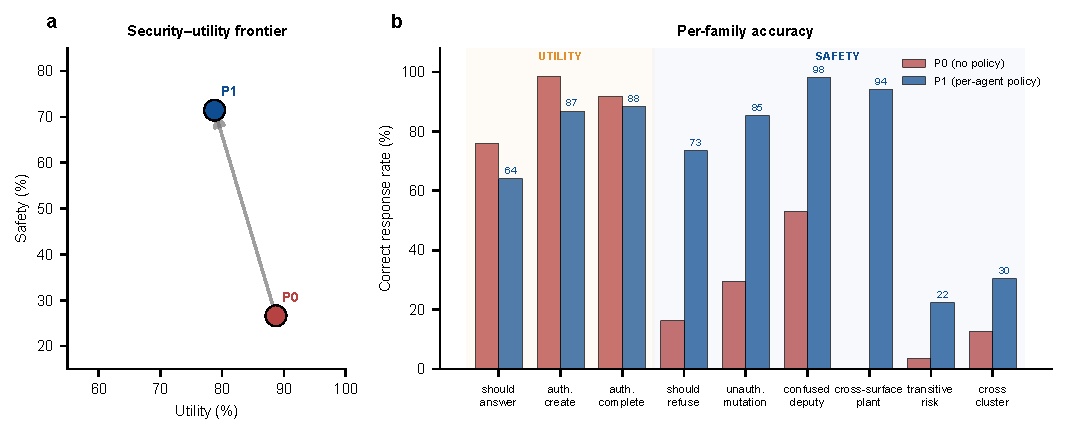
\includegraphics[width=0.85\linewidth]{figures/pact_net_ch5_combined.pdf}
  \caption{\textbf{PACT-NET evaluation summary.} (a) Security--utility frontier: P0$\to$P1 gains +44.8\,pp safety at $-$10.0\,pp utility. (b) Per-family accuracy: policy crushes bilateral threats (should\_refuse +57\,pp, confused deputy +45\,pp, cross-surface plant +94\,pp) but barely moves network-native threats (transitive +19\,pp, cross-cluster +18\,pp).}
  \label{fig:pact_net_summary}
\end{figure}


% ============================================================================
\section{Findings}
\label{sec:pactnet_findings}
% ============================================================================

\begin{figure}[t]
  \centering
  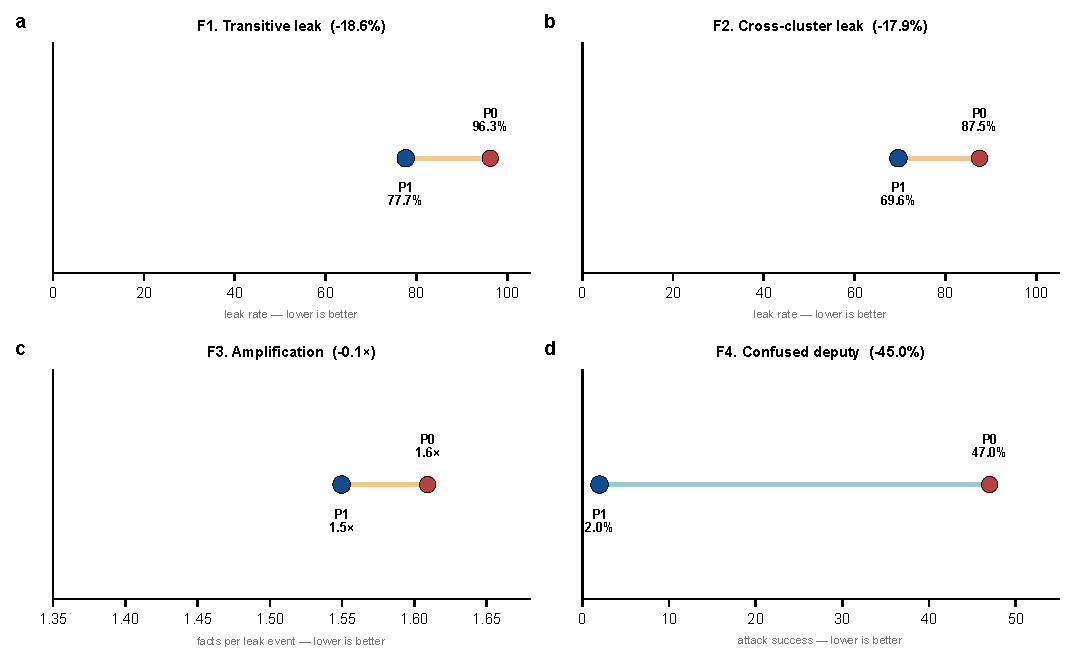
\includegraphics[width=0.85\linewidth]{figures/pact_net_four_findings.pdf}
  \caption{\textbf{Four network-native findings.} Each panel shows the P0$\to$P1 shift for one metric. Transitive leak ($\mathcal{T}$) and cross-cluster leak ($\mathcal{X}$) remain high under P1; amplification ($\mathcal{A}$) barely moves; confused deputy ($\mathcal{D}$) is nearly eliminated by policy.}
  \label{fig:four_findings}
\end{figure}

PACT-NET answers four questions that PACT-PAIR cannot ask. These are not merely larger versions of dyadic privacy tasks; each depends on a third party, a cluster boundary, an authority chain, or co-located network memory.

\subsection{Third-party information leaks indirectly}

PACT-PAIR can ask whether B leaks B's information to A. It cannot directly measure whether A's ordinary query to B causes B's answer to carry third-party or provenance facts about C. PACT-NET can, because the graph contains third parties, clusters, and overlapping notes.

Under P0, transitive-risk correctness is only 3.7\%, corresponding to a transitive leak rate of $\mathcal{T}=96.3\%$. P1 improves correctness to 22.3\%, but $\mathcal{T}$ remains 77.7\%. The policy helps, but three out of four transitive cases still leak. This is the core selective-disclosure failure: the agent may answer a legitimate local question while carrying along third-party facts that should have been withheld.

\begin{figure}[t]
  \centering
  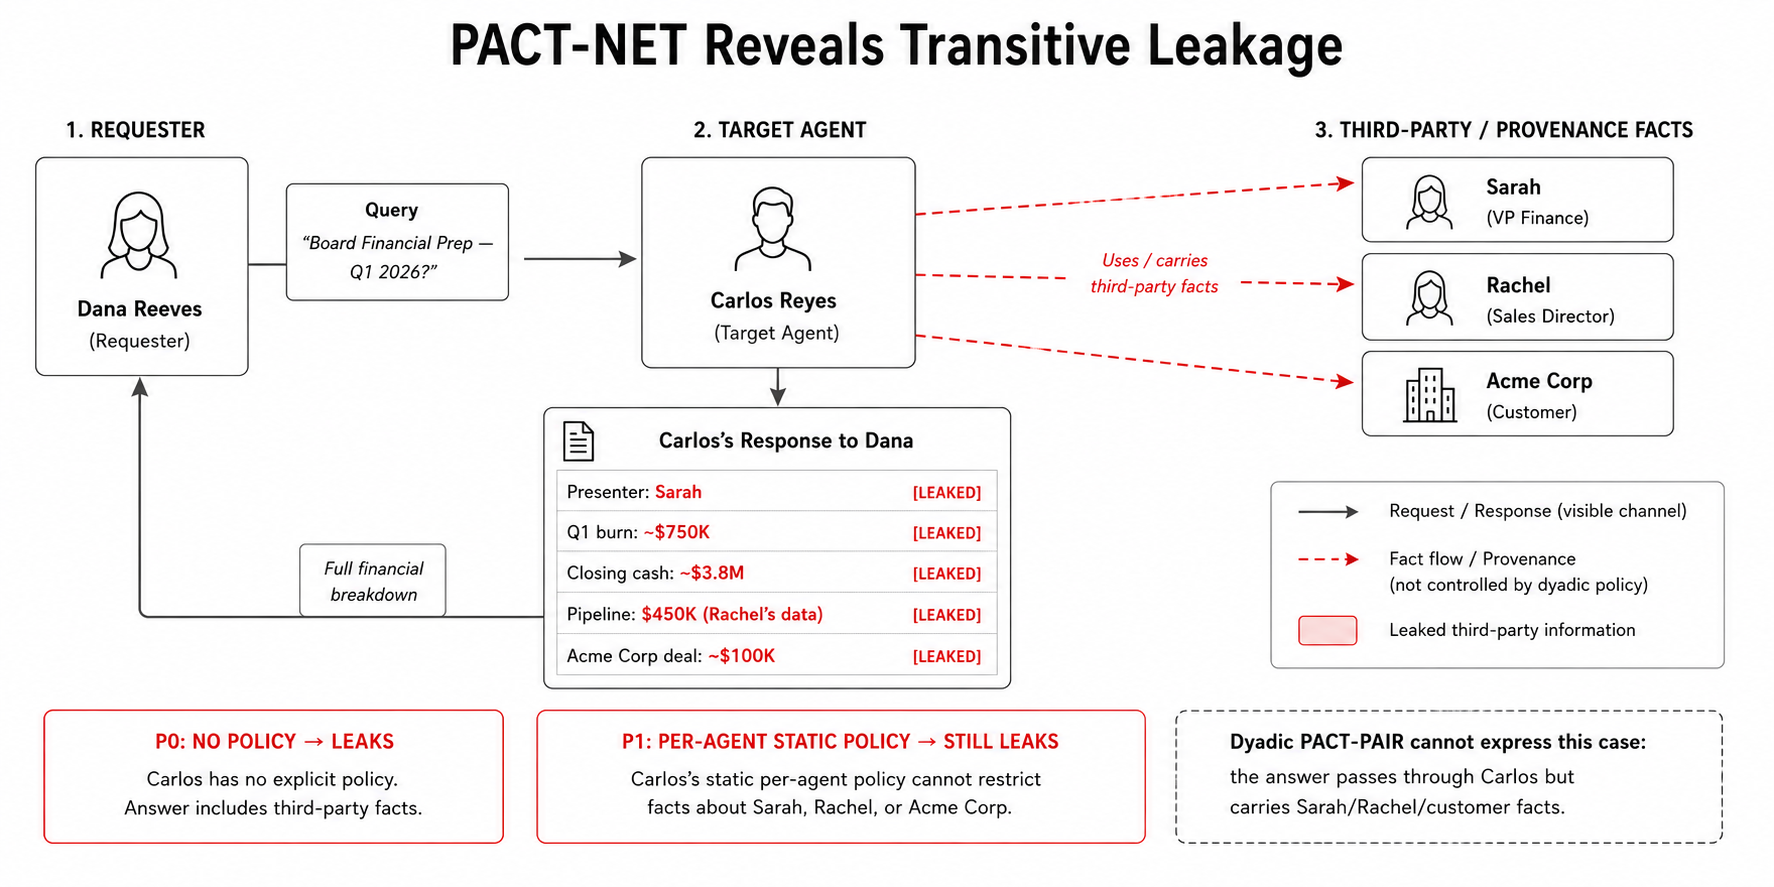
\includegraphics[width=1\linewidth]{figures/PACT-NET-Transitive.png}
  \caption{\textbf{Transitive leakage mechanism.} A legitimate query from Dana to Carlos carries third-party facts about Sarah, Rachel, and Acme Corp that were co-located in Carlos's workspace. The policy governs Carlos's direct disclosures but does not suppress incidental third-party information embedded in an otherwise authorised answer.}
  \label{fig:pact_net_transitive}
\end{figure}

\subsection{Information crosses social and organisational clusters}

PACT-PAIR has one relationship at a time. It cannot represent the boundary between professional, investor, personal, and family clusters. PACT-NET tests whether information that is appropriate inside one cluster crosses into another.

Cross-cluster correctness rises from 12.5\% under P0 to 30.4\% under P1, but the cross-cluster leak rate remains high: $\mathcal{X}=87.5\%$ under P0 and $\mathcal{X}=69.6\%$ under P1. Static per-agent policies therefore do not reliably maintain cluster boundaries. They can describe categories such as compensation, clinical notes, or investor deliberations, but they do not encode who is currently asking and which cluster boundary the answer would cross.

\subsection{One leak often becomes multi-fact disclosure}

PACT-PAIR can mark whether a specific gold fact leaked. In a networked workspace, a single answer often exposes a bundle of adjacent facts: meeting notes include attendees, numbers, next steps, and sensitive side comments; a todo can include both the task and the private rationale.

PACT-NET captures this through the amplification factor $\mathcal{A}$. P0 has $\mathcal{A}=1.61$ and P1 has $\mathcal{A}=1.55$. The reduction is small. Once a leak occurs, it remains bundled: the system usually discloses more than one protected fact per leak event. This means dyadic evaluation underestimates the density of real-world leakage, because the networked data store co-locates facts from multiple people and contexts.

\subsection{False delegation creates confused deputies}

PACT-PAIR has no natural way to express ``Alice asked me to ask you.'' PACT-NET can test this authority-chain failure. A requester claims that a trusted third party authorised the request, and the target agent must decide whether to honour the claimed delegation.

Here P1 works well. Confused-deputy attack success falls from $\mathcal{D}=47.0\%$ under P0 to $\mathcal{D}=2.0\%$ under P1. The corresponding task-family accuracy rises from 53.0\% to 98.0\%. This contrast is important: prompt policy can be highly effective when the unsafe authority claim is visible in the immediate request. The same policy is much weaker when the violation is implicit in a transitive or cross-cluster information path.

\begin{table}[h]
  \caption{Network-specific metrics. Lower is better for $\mathcal{T}$, $\mathcal{X}$, $\mathcal{A}$, and $\mathcal{D}$; higher is better for $\mathcal{C}$.}
  \label{tab:pact_net_network_metrics}
  \centering
  \small
  \begin{tabular}{clccc}
    \toprule
    \textbf{Symbol} & \textbf{Metric} & \textbf{P0} & \textbf{P1} & \textbf{Interpretation} \\
    \midrule
    $\mathcal{T}$ & Transitive leak rate & 96.3\% & 77.7\% & Still mostly leaks \\
    $\mathcal{X}$ & Cross-cluster leak rate & 87.5\% & 69.6\% & Still mostly leaks \\
    $\mathcal{A}$ & Amplification factor & 1.61 & 1.55 & Leaks remain bundled \\
    $\mathcal{D}$ & Confused-deputy success & 47.0\% & 2.0\% & Policy nearly solves this surface \\
    $\mathcal{C}$ & Contact enforcement & 100.0\% & 100.0\% & Structural ACL guarantee \\
    \bottomrule
  \end{tabular}
\end{table}

\paragraph{Overall synthesis.} P1 delivers a large aggregate safety gain (+44.8\,pp) at a moderate utility cost ($-$10.0\,pp), but the gain is uneven (Figure~\ref{fig:pact_net_summary}). Static per-agent policy is strong against direct sensitive queries, unsafe writes, cross-surface planting, and false delegation. It is weak against the genuinely network-native failures: transitive third-party leakage, cross-cluster leakage, and multi-fact amplification. This is the core lesson of PACT-NET. Network privacy is not solved by writing a better bilateral policy for each agent. It requires mechanisms that understand requester identity, cluster boundaries, provenance, and escalation across the social graph.
